%Créé par Claudine Allen en collaboration avec Jérémie Guilbert
%Dernière modification JG: 11 novembre 2020
%Dernière modification CA: 15 novembre 2020
%******************
%ToDo
%- Section 3.1 de résonance: éventuellement commenter dans l'analogie du système masse-ressort que la masse est une constante de proportionnalité dans l'inertie qte de mvt et non pas une propriété intrinsèque de la matière qui est plutôt le nbre d'atomes et masse étalonnée sur isotope carbone. J'ai déjà lu un super texte là-dessus, à retrouver.
%- Section 3.1 de résonance: dans le coin du retour vers un EDO non homogène vu le besoin d'un ampli-op pour forcer les oscillations, ajouter plus clairement (graphes et tout) l'effet du terme d'entretien à la résonance qui fait dépasser l'amplitude initiale (retour de l'énergie des composants dans le circuit, répartition différente de l'énergie dans le temps) en contraste à l'amortissement en l'absence de termes d'entretien. Capsule vidéo de cet effet dans un circuit RLC avec vieil oscillo analogique, en connexion avec atelier filtre itou, et système masse-ressort du jouet paddle ball!
%
\RequirePackage[l2tabu, orthodox]{nag} %Check for obsolete commands
\documentclass[canadien,12pt,oneside,letterpaper]{article}
%
%-----------------------------------------------------
%Loading packages
%
\usepackage[utf8]{inputenc}
\usepackage[T1]{fontenc}
\usepackage[canadien]{babel}
\usepackage{lmodern}
\usepackage{textcomp}
\usepackage{amsmath,amssymb}
\usepackage{siunitx}
\usepackage[svgnames]{xcolor}
\usepackage{hyperref}
\usepackage[all]{hypcap}
\usepackage{graphicx}
\usepackage[americanvoltages,americancurrents,siunitx]{circuitikz}
\usetikzlibrary{babel}
\usepackage{pgfplots}
\pgfplotsset{compat=1.15}
\usepackage{mathrsfs}
\usetikzlibrary{arrows}
\usepackage{caption}
%\usepackage{subcaption}
\usepackage{subfig}
\usepackage[letterpaper,headheight=15pt]{geometry}
\usepackage{fancyhdr}
\usepackage{setspace}
%
\captionsetup{font=small,labelfont=bf,margin=0.1\textwidth}
\pagestyle{myheadings}
\markboth{PHY-2002/GPH-2006~---~Oscillateurs électroniques}{PHY-2002/GPH-2006~---~Oscillateurs électroniques}

\begin{document}
 
\title{\textbf{Complément}\\Oscillateurs électroniques}
\author{Jérémie Guilbert \& Claudine Allen}
\date{}
\maketitle

% En plus d'atténuer les signaux alternatifs dans une bande de fréquences donnée, les filtres peuvent être utilisés en combinaison avec des amplificateurs opérationnels afin de générer activement des signaux oscillants à des fréquences voulues. La génération de ces signaux fait intervenir la fonction de comparateur d'un ampli-op afin de contrôler le cycle de charge-décharge d'un condensateur, puis celle d'amplification avec rétroaction afin de sélectionner la fréquence d'oscillation avec un filtre passe-bande. Des fonctions d’intérêt pour les circuits oscillateurs étudiés sont d’actionner un transducteur afin d’obtenir des ondes mécaniques, ou encore de définir un étalon de temps lorsque l’oscillation est pratiquement harmonique avec une seule fréquence.

\section{Oscillateur à relaxation avec comparateur}
\begin{figure}[h]
\centering
\begin{circuitikz} \draw
(0,0) node[op amp](opamp){}
(opamp.+) to[short] (-1.2,-0.5) to[short] (-1.2,-2.2)
(opamp.-) to[short] (-1.2,0.5) to[short] (-1.2,2.2)
(opamp.out) to[short,-o] (2.1,0) node[right]{$v_{\mathrm{out}}$}
(opamp.down) ++ (0,-0.5) node[below]{$-5$~V} -- (opamp.down)
(opamp.up) ++ (0,0.5) node[above]{5~V} -- (opamp.up)
(-4,2.2) node[ground]{} to[C=$C$] (-1.2,2.2) to[R=$R$] (1.6,2.2) to[short] (1.6,-2.2) to[R=10~k$\Omega$] (-1.2,-2.2) to[R=10~k$\Omega$] (-4,-2.2) node[ground]{}
;\end{circuitikz}
\caption{\label{sch-osc-relax}Oscillateur à relaxation avec comparateur}
\end{figure}
%Ancienne légende de la figure 1
Le circuit illustré à la figure \ref{sch-osc-relax}
est basé sur l'utilisation de la fonction comparateur de l'ampli-op qui permet de contrôler le cycle de charge-décharge d'un condensateur afin de générer des oscillations à une fréquence déterminée par les valeurs des composants du circuit. Le condensateur qui se charge cause éventuellement l'entrée inverseuse de l'amplificateur opérationnel à dépasser celle non inverseuse et la tension de sortie de ce comparateur tombe alors négative, renversant ainsi la polarité appliquée sur le condensateur. Celui-ci se décharge maintenant jusqu'à ce que l'entrée inverseuse repasse sous celle non inverseuse et remet la sortie positive pour recommencer le cycle. 

\section{Oscillateur harmonique à rétroaction - pont de Wien}
\begin{figure}[h]
\centering
\begin{circuitikz} \draw
(0,0) node[op amp](opamp){}
(opamp.+) to[short] (-1.2,-0.5) to[short] (-1.2,-2.2)
(opamp.-) to[short] (-1.2,0.5) to[short] (-1.2,2.2)
(opamp.out) to[short,-o] (2.1,0) node[right]{$v_{\mathrm{out}}$}
(opamp.down) ++ (0,-0.5) node[below]{$-5$~V} -- (opamp.down)
(opamp.up) ++ (0,0.5) node[above]{5~V} -- (opamp.up)
(-4,2.2) node[ground]{} to[R=1~k$\Omega$] (-1.2,2.2) to[R=10~k$\Omega$] (1.6,2.2) to[short] (1.6,0) to[C=$C$] (1.6,-2.2) to[R=$R$] (-1.2,-2.2)
(-1.2,-2.2) to[C=$C$] (-3,-2.2) node[ground]{} to[R=$R$] (-3,-0.5) to[short] (-1.2,-0.5)
;\end{circuitikz}
\caption{\label{sch-osc-Wien}Oscillateur harmonique à rétroaction - pont de Wien}
\end{figure}
Le circuit à la figure \ref{sch-osc-Wien} ci-dessus utilise l'ampli-op en mode rétroaction afin de sélectionner la fréquence du signal qui entrera à l'entrée non inverseuse au moyen d'un filtre passe-bande, permettant par le fait-même de contrôler la fréquence des oscillations à la sortie.

Le signal à l'entrée non inverseuse, qui n'est \textit{a priori} que du bruit car aucune source n'est présente, est amplifié puis passe au travers d'un pont de Wien qui le filtre. Le signal ainsi filtré retourne ensuite à l'entrée de l'amplificateur pour être à nouveau amplifié et filtré, et ainsi de suite, \textit{ad infinitum}. Le pont de Wien est \textit{grosso modo} l'addition d'un filtre passe-bas et d'un filtre passe-haut pour former un filtre passe-bande. La fréquence du signal de sortie est alors $f=\left(2\,\pi\,R\,C\right)^{-1}$. L'amplitude finale du signal est fixée par la source d'alimentation de l'ampli-op. % Cet oscillateur doit son oscillation au chargement/déchargement du condensateur qui relie l'entrée non inverseuse de l'amplificateur au \textit{ground}.

\section{Oscillateur harmonique à rétroaction (LC)}
%Ancienne intro partie 3
Un autre oscillateur reposant sur le même principe de filtrage et amplification en boucle du signal est l'oscillateur~LC. Vous avez étudié au dernier atelier le filtre~RLC passe-bande dont le gain et la fréquence de résonance peuvent être déterminés analytiquement à partir des valeurs de résistance~$R$, d'inductance~$L$ et de capacitance~$C$ du circuit. On peut donc remplacer le pont de Wien du dernier oscillateur par un circuit~RLC afin d'obtenir, avec un choix judicieux des composants du circuit, une fréquence de résonance et un gain quelconques. 

\subsection{Résonance et équation différentielle des oscillateurs}
On peut déterminer la fréquence de résonance $\omega_0=2\pi f_0$ d'un circuit oscillatoire passif en déterminant l'équation différentielle linéaire décrivant la tension ou le courant du circuit au point d'intérêt. Pour ce faire, le principe demeure le même que l'analyse de tout circuit réactif tel que modélisé précédemment à l'aide de la transformation de Laplace, mais ici l'accent est mis sur l'équation différentielle ordinaire~(EDO) de départ afin de mieux faire ressortir les liens avec la théorie étudiée dans vos cours de physique mathématique. Les étapes générales d'analyse sont donc
\renewcommand{\labelenumi}{\Roman{enumi}.}
\begin{enumerate}
    \item déterminer le modèle gouvernant le circuit à partir des lois de Kirchhoff,
    \item substituer les relations constitutives tension/courant pour chacun des composants du circuit, soit
    \begin{equation} \label{eq:RelCon}
    \begin{split}
        \text{résistance : } v_R(t) &= R\,i(t) \quad\text{ou}\quad i_R(t)=\frac{v_R(t)}{i_R(t)}\,,\\
        \text{condensateur : } i_C(t) &= C\,\frac{\mathrm{d}v(t)}{\mathrm{d}t} \quad\text{ou}\quad v_C(t) = v(0)+\frac{1}{C}\int_0^ti(t')\,dt'\,,\\
        \text{bobine : } v_L(t) &= L\,\frac{\mathrm{d}i(t)}{\mathrm{d}t} \quad\text{ou}\quad i_L(t)  = i(0)+\frac{1}{L}\int_0^tv(t')\,dt'\,,
    \end{split}
    \end{equation}
    \item exprimer l'équation différentielle en termes de la variable d'intérêt~$i(t)$ ou~$v(t)$ au point désiré et résoudre l'équation.
\end{enumerate}

\begin{figure}[h]
\centering
\begin{circuitikz} \draw
(0,3) to[V, l_=$V_S$] (0,0)
(0,3) to[C=$C$] 
(3,3) to[R=$R$,i>^=$I$] 
(3,0) to[L=$L$] (0,0);
\end{circuitikz}
\caption{Circuit RLC en série.}
\label{circuitRLC-serie}
\end{figure}

L'oscillateur le plus simple est le circuit~RLC en série de la figure~\ref{circuitRLC-serie}. En effet, le comportement transitoire du courant~$i(t)$ dans l'unique maille s'analyse ainsi:
\begin{enumerate}
    \item $v_S(t)=v_C(t)+v_R(t)+v_L(t)$ avec la loi des mailles de Kirchhoff,
    \item $\displaystyle v_S(t)=v(0)+\frac{1}{C}\int_0^ti(t')\,dt'+Ri(t)+L\frac{\mathrm{d}i(t)}{\mathrm{d}t}$ avec les relations constitutives,
%\end{enumerate}
%Si on suppose maintenant que la source produit une tension constante, on a, en prenant la dérivée de l'équation précédente, 
%\begin{enumerate}
%  \setcounter{enumi}{2}
  \item $\displaystyle \frac{\mathrm{d}v_S(t)}{\mathrm{d}t} = L\,\frac{\mathrm{d}^2i(t)}{\mathrm{d}t^2}+R\,\frac{\mathrm{d}i(t)}{\mathrm{d}t}+\frac{1}{C}\,i(t)$ en prenant la dérivée.
\end{enumerate}
En exprimant cette équation sous forme canonique $\ddot x(t) + 2\alpha\,\dot x(t) + \omega_0^2\,x(t) = f(t)$ avec un coefficient unitaire du terme en dérivée seconde et des coefficients constants pour les termes subséquents, on a bien une~EDO d'ordre~2 \textit{non homogène}
\begin{equation}\label{eq:RCL}
    \frac{\mathrm{d}^2i(t)}{\mathrm{d}t^2}+\frac{R}{L}\,\frac{\mathrm{d}i(t)}{\mathrm{d}t}+\frac{1}{LC}\,i(t) = \frac{\mathrm{d}v_S(t)}{\mathrm{d}t}\,.
\end{equation}

\begin{figure}[h]
    \centering
    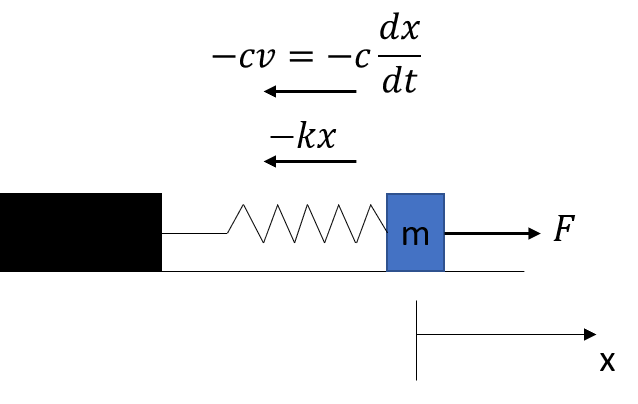
\includegraphics[width=0.55\textwidth]{Labos-Complements/Lab08/masse_ressort.png}
    \caption{Système masse-ressort sur une surface sans friction dans un milieu visqueux. Trois forces agissent sur la masse $m$ au bout du ressort: la force de rappel dictée par la constante de rappel du ressort~$k$, une force de frottement fluide proportionnelle à la vitesse de la masse $v(t)=\dot x(t)$, dont le coefficient de proportionnalité est l'amortissement~$c$, ainsi qu'une force extérieure~$F$.}
    \label{fig:systeme_masse_ressort}
\end{figure}
Pour mieux visualiser la signification de chacun des termes de cette équation, il est utile d'utiliser une analogie avec un système plus intuitif, le système masse-ressort illustré à la figure~\ref{fig:systeme_masse_ressort}. À partir des forces identifiées sur la figure, l'équation du mouvement pour un objet au bout d'un ressort dans un milieu visqueux est 
\begin{equation}
    %\begin{split}
      \sum \mathcal{F} = m\frac{\mathrm{d}^2x}{\mathrm{d}t^2} = -c\frac{\mathrm{d}x}{\mathrm{d}t}-kx+F,% \\
     % &\Rightarrow \frac{d^2x}{dt^2}+\frac{c}{m}\frac{dx}{dt}+\frac{k}{m}x = F.
    %\end{split}
\end{equation}
avec la forme canonique 
\begin{alignat}{2}\label{eq:masse_ressort}
    \ddot x(t) + 2\alpha\,\dot x(t) + \omega_0^2\,x(t) = f(t)\notag\\
    \frac{\mathrm{d}^2x(t)}{\mathrm{d}t^2} + \frac{c}{m}\,\frac{\mathrm{d}x(t)}{\mathrm{d}t} + \frac{k}{m}\,x(t) = F(t).
\end{alignat}

Cette forme met en évidence l'association terme à terme d'abord de la résistance~$R$ du circuit~RLC au coefficient d'amortissement fluide~$c$, celui-ci générant une force de frottement qui s'oppose au mouvement de la masse de façon proportionnelle à sa vitesse, similairement à la résistance qui crée une opposition au courant proportionnelle à sa dérivée temporelle. De même, les paramètres~$L$ et~$C$ peuvent être respectivement associés à la masse $m$ et à l'inverse de la constante de rappel du ressort~$k$. La table~\eqref{tab:equiv_masse_ressort} résume ces équivalences mathématiques entre les coefficients constants des EDO. %En l'absence de résistance, le système sera donc non-amorti et oscillera à la fréquence $\omega_0=\frac{1}{\sqrt{LC}}$. Si la résistance est non-nulle, la fréquence d'oscillation sera amortie et sera plutôt de $\sqrt{w_0^2-\alpha^2}=\sqrt{\frac{1}{LC}-\left(\frac{R}{L}\right)^2}$.

\begin{table}[h]
\centering
\begin{tabular}{c|ccc}
\hline
Dynamique & Amortissement & Oscillation & Terme d'entretien \\
Terme associé & $\mathrm{d}x(t)/\mathrm{d}t$ & $x(t)$ & 1\\
\hline
\textbf{canonique} & $2\alpha$ & $\omega_0$ & f(t)\\
\textbf{masse-ressort} & $\displaystyle\frac{c}{m}$ & $\displaystyle\sqrt{\frac{k}{m}}$ & $F(t)$ \\
\textbf{circuit RLC} & $\displaystyle\frac{R}{L}$ & $\displaystyle\frac{1}{\sqrt{LC}}$ & $\displaystyle\frac{\mathrm{d}v_S(t)}{\mathrm{d}t}$ \\
\hline
\end{tabular}
\caption{Équivalences entre les coefficients des EDO de 2\textsuperscript{e} ordre qui modélisent la physique d'un système masse-ressort et d'un circuit RLC.}
\label{tab:equiv_masse_ressort}
\end{table}

% S'il n'y a pas de force $F$ qui entretient le mouvement, l'équation \ref{eq:masse_ressort} a la même forme que l'équation pour le courant du circuit RLC avec une source constante. Cette équation, exprimée sous la forme canonique
% \begin{equation}\label{eq:canonique}
%     \frac{d^2I(t)}{dt^2}+2\alpha\frac{dI(t)}{dt}+\omega_0^2I(t) = 0,
% \end{equation}
Lorsque le terme d'entretien est nul, la tension d'alimentation $v_s$ pouvant même être constante, l'EDO devient homogène et la dynamique transitoire est la même pour le courant dans le circuit~RLC et pour la position dans le système masse-ressort. La solution générale du cas $\frac{\alpha}{\omega_0}<1$ se simplifie à
\begin{equation}\label{eq:sol_gen}
   i(t) = x(t) = Ae^{-\alpha t}\sin\left(\sqrt{\omega_0^2-\alpha^2}\:t+\varphi\right), 
\end{equation}
où $A$ et $\varphi$ sont des constantes déterminées par les conditions initiales du système\footnote{La fonction~\eqref{eq:sol_gen} correspond à une superposition de deux solutions linéairement indépendantes comme il se doit pour une EDO homogène d'ordre~2. La fonction harmonique est obtenue à l'aide d'identités trigonométriques remaniant les coefficients en constantes d'amplitude $A$ et de phase $\varphi$.}. Cette fonction représente l'oscillation de la variable dépendante $i(t)$ ou $x(t)$ à la fréquence $\sqrt{\omega_0^2-\alpha^2}$. L'amplitude de l'oscillation, initialement de $A$, décroît de façon exponentielle avec le temps à un taux dicté par la constante $\alpha$ inversement proportionnelle à constante de temps du circuit $\tau=1/\alpha$. En l'absence de dissipation d'énergie par résistance ou frottement, le système n'est plus amorti et oscillera à sa \textbf{fréquence de résonance} $\mathbf{\omega_0}$, soit $\frac{1}{\sqrt{LC}}$ pour le circuit RLC et $\sqrt{\frac{k}{m}}$ pour le système masse-ressort. 

%En comparant terme à terme les équations \ref{eq:RCL}, \ref{eq:masse_ressort} et \ref{eq:canonique} avec cette solution, on observe une équivalence entre les termes résumée au tableau \ref{tab:equiv_masse_ressort}. 

%Si la résistance est non-nulle, la fréquence d'oscillation sera amortie et sera plutôt de $\sqrt{w_0^2-\alpha^2}=\sqrt{\frac{1}{LC}-\left(\frac{R}{L}\right)^2}$.
%La résolution de l'équation homogène décrite ici permet de trouver la fréquence de résonance d'un circuit. 

Il faut insister sur le fait que les oscillations naturelles dans le circuit~RLC sont toujours transitoires, elles ne peuvent pas perdurer beaucoup plus longtemps que la constante de temps $\tau$ du circuit. En effet, même un circuit~LC (\textit{tank or tuned circuit}) sans composant résistif dissipera de la puissance hors du circuit puisque les fils ne sont pas idéaux avec une résistivité intrinsèque non nulle. C'est pourquoi un composant actif, donc alimenté comme l'ampli-op, est nécessaire dans la conception d'oscillateurs électroniques et que l'analyse doit aussi considérer le régime permanent maintenu par un terme d'entretien non nul, tel que vu en classe et dans le complément \textit{Analyse fréquentielle}. Les relations constitutives~\eqref{eq:RelCon} permettent d'obtenir directement le comportement aussi oscillatoire de la différence de potentiel aux bornes de chaque composant et on peut alors retrouver la réponse en fréquence du circuit~RLC à l'aide de la transformée de Fourier. Toutefois, la présence d'un ampli-op demanderait un système d'EDO non linéaires, non homogènes et couplées pour complètement représenter le circuit, d'où on se tourne plutôt vers un modèle approximatif de l'ampli-op tel qu'introduit dans le complément \textit{Amplificateurs} et vers le diagramme de Bode du gain pour le circuit~RLC, soit un filtre passe-bande. 

%Pour déterminer la réponse en fréquence, c'est-à-dire la valeur du gain en fonction de la fréquence d'oscillation du signal d'entrée $V_S(t)$, il faut résoudre l'équation non-homogène. Ceci est habituellement réalisé en calculant la fonction de transfert du système directement dans l'espace des fréquences avec les expressions pour l'impédance des composants, tel que détaillé dans le complément \textit{Analyse fréquentielle}.

 %Noter qu'à partir de la solution dérivée pour le courant circulant dans le circuit RLC en série, on pourrait obtenir obtenir des équations pour la tension aux bornes de chacun des composants à partir des relations tension/courant. Par exemple, si on désire connecter une charge sur la bobine, on pourrait déterminer la tension à l'entrée de la charge en connaissant $I(t)$ et sachant que $V_L(t) = L\frac{dI(t)}{dt}$.

\section{Oscillateur avec la puce 555}
%Ancienne sous-section
\begin{figure}[h]
\centering
\begin{circuitikz} \draw[thick]
(0,0) to[short] (0,0.5) node[right]{4} to[short,*-*] (0,1.5) node[right]{3} to[short] (0,2.5) node[right]{2} to[short,*-*] (0,3.5) node[right]{1} to[short] (0,4) to[short] (3,4) to[short] (3,3.5) node[left]{8} to[short,*-*] (3,2.5) node[left]{7} to[short] (3,1.5) node[left]{6} to[short,*-*] (3,0.5) node[left]{5} to[short] (3,0) to[short] (0,0)
{[anchor=east] (0,3.5) node{\textbf{GND}} (0,2.5) node{\textbf{TRIG}} (0,1.5) node{\textbf{v$_{\text{out}}$}} (0,0.5) node{\textbf{RESET}}}
{[anchor=west] (3,3.5) node{\textbf{v$_{\text{cc}}$}} (3,2.5) node{\textbf{DISCH}} (3,1.5) node{\textbf{THRES}} (3,0.5) node{\textbf{CONT}}}
;\end{circuitikz}
\caption{\label{sch-555}Schéma des ports d'entrée et sortie d'une puce 555.}
\end{figure}
La puce 555 est un circuit intégré (figure \ref{sch-555}) souvent utilisé en électronique analogique pour, entre autres, bâtir des oscillateurs. Les niveaux de déclenchement (\textit{trigger}) et de seuil (\textit{threshold}) valent respectivement un tiers et deux tiers de l'alimentation \textbf{v$_{\text{cc}}$}. Lorsque l'entrée \textbf{TRIG} est inférieure au niveau de déclenchement, la sortie de la puce \textbf{v$_{\text{out}}$} vaut \textbf{v$_{\text{cc}}$}. Lorsque l'entrée \textbf{TRIG} est supérieure au niveau de déclenchement et qu'en plus l'entrée \textbf{THRES} est supérieure au niveau de seuil, alors la sortie devient nulle. Lorsque la sortie devient nulle, un court-circuit se fait entre l'entrée \textbf{DISCH} (\textit{discharge}) et la mise à la terre. La table \ref{table-555} résume ce fonctionnement.

\begin{table}[h]
\centering
\begin{tabular}{|c|c|c|}
\hline
\textbf{TRIG} & \textbf{THRES} & \textbf{OUT} \\
\hline
$<\frac{1}{3}$\textbf{v$_{\text{cc}}$} & --- & \textbf{v$_{\text{cc}}$} \\
\hline
$>\frac{1}{3}$\textbf{v$_{\text{cc}}$} & $>\frac{2}{3}$\textbf{v$_{\text{cc}}$} & 0 \\
\hline
$>\frac{1}{3}$\textbf{v$_{\text{cc}}$} & $<\frac{2}{3}$\textbf{v$_{\text{cc}}$} & Conserve l'état \\
\hline
\end{tabular}
\caption{\label{table-555}Sortie d'une puce 555 en fonction des tensions aux entrées \textbf{TRIG} et \textbf{THRES}.}
\end{table}

La figure~\ref{sch-alarme-1} illustre comment utiliser la puce 555 pour générer un signal oscillant à une fréquence précise. Initialement, lorsque le bloc d'alimentation s'allume, la tension à l'entrée \textbf{TRIG} est basse, donc la sortie est élevée ($v_{\mathrm{out}}=v_{\mathrm{s}}=\mathbf{v_{\text{cc}}}$) et le condensateur de capacité $C$ se charge avec une constante de temps $\tau=\left(R_A+R_B\right)\,C$. La tension aux bornes du condensateur, \textit{i.e.} la tension aux terminaux \textbf{TRIG} et \textbf{THRES}, augmente jusqu'à atteindre le niveau de seuil, soit $\frac{2}{3}\,v_{\mathrm{s}}$. À ce moment, la sortie devient basse ($v_{\mathrm{out}}=0$~V), le terminal \textbf{DISCH} devient mis à la terre et le condensateur se décharge avec une constante de temps plus petite $\tau=R_B\,C$. Lorsque la différence de potentiel aux bornes du condensateur a diminué jusqu'à atteindre $\frac{1}{3}\,v_{\mathrm{s}}$, alors la sortie redevient élevée, le terminal \textbf{DISCH} est déconnecté de la masse et le condensateur recommence à se charger. Ainsi, la sortie passe de 0~V à $v_{\mathrm{s}}$ puis retourne à 0~V et ainsi de suite, avec une période de $T=\mathrm{ln}\!\left(2\right)\left(R_A+2\,R_B\right)C$\label{eq:alarme}.

\begin{figure}[H]
\centering
\begin{circuitikz} \draw[thick]
(0,0) to[short,-*] 
(0,1) node[right]{2} to[short] 
(0,2) node[right]{6} to[short,*-*] 
(0,3) node[right]{7} to[short] 
(0,4) to[short] 
(1,4) node[below]{4} to[short,*-*] 
(2,4) node[below]{8} to[short] 
(3,4) to[short] 
(3,3) node[left]{3} to[short,*-*] 
(3,1) node[left]{5} to[short] 
(3,0) to[short,-*] 
(1.5,0) node[above]{1} to[short] (0,0)
;\draw
(3,3) to[short,-o] 
(3.5,3) node[right]{$v_{\mathrm{out}}$}
(1.5,0) to[short] (1.5,-0.5)
(-2,-0.5) to[C=$C$] 
(-2,1) to[R=$R_B$] 
(-2,3) to[R=$R_A$] 
(-2,5) to[short] (2,5)
(-2,1) to[short] (0,1)
(-1,1) to[short] 
(-1,2) to[short] (0,2)
(-2,3) to[short] (0,3)
(1,4) to[short] (1,5)
(2,4) to[short] (2,5)
(-4,5) to[V, l_=$v_{\mathrm{s}}$] (-4,-0.5)
(-4,-0.5) node[ground]{} 
(-4,5) to[short] (-2,5)
(-4,-0.5) to[short] (1.5,-0.5)
;\end{circuitikz}
\caption{Circuit d'une puce 555 en mode astable. Les numéros des entrées de la puce sont définis à la figure~\ref{sch-555}.}
\label{sch-alarme-1}
\end{figure}

\section{Modification de largeur d'impulsion (PWM)}
La modification de la largeur d'impulsion, ou \textit{pulse width modulation} (PWM) en anglais, est une technique principalement utilisée pour contrôler la puissance acheminée à une charge quelconque. Par exemple, celle-ci permet de contrôler la vitesse d'un moteur DC ou l'intensité d'une lumière DEL. Supposons un signal carré périodique tel qu'illustré à la figure []. Pour une période donné, on appelle rapport cyclique ou \textit{duty cycle} la fraction de la période où la tension est non-nulle dans le signal. En définissant la période du signal par:
$$T = T_{on} + T_{off},$$
le rapport cyclique est donné par:
$$\text{Rapport cyclique} = \frac{T_{on}}{T_{on} + T_{off}}$$
Comme le nom l'indique, en PWM on fait varier la largeur de l'impulsion et par de fait même le rapport cyclique. C'est en faisant varier celui-ci qu'on peut choisir la tension effective du signal et contrôler par exemple l'intensité lumineuse d'une lumière DEL. Cette tension est donnée par:
$$V_{eff} = V_{on} \times \text{Rapport cyclique}$$
Ainsi, pour le cas de la lumière, l'intensité sera proportionnelle à la tension efficace. En effet, si on a un signal avec une valeur maximale de 5 V, même si la lumière reçoit effectivement 5 V pendant un certain temps de la période du signal, si on utilise une fréquence assez élevée l'oeil humain percevra une diminution de l'intensité lumineuse lorsqu'on fait diminuer le rapport cyclique du signal. Pour le cas d'un moteur DC, d'une manière similaire, si on a une fréquence de signal suffisamment élevé, le moment où la tension est nulle est négligeable et donc l'effet net de la modification de la largeur d'impulsion est de contrôler la vitesse du moteur. Certains pourraient se demander quel est l'avantage d'utiliser le PWM à la place de tout simplement diminuer ou augmenter la tension d'un signal DC. Pour certains composants comme le moteur, la tension sera tout simplement insuffisante pour le faire fonctionner à partir d'un certain point. De plus, il n'y a souvent pas de corrélation linéaire entre la tension et le output d'un composant quelconque. La modification de la largeur d'impulsion est donc supérieure pour contrôler précisément le \textit{output} voulu. 

\end{document}